\chapter{Stiffness Calculation}
\label{ch:Stiff_Calc}



YOOOOOOO WAGWAN THIS IS SOME COOL PLACEHOLDER TEXT

\textcolor{orange}{I LOOOOOOVVVEEE it!! \\
    -The Burger King (Louisville, Kentucky 1407)\\
        -King Arthur (Came a lot, some castle 200 b.c.)\\
            -Cleopatra (Middle Earth, On a T-Rex 64 Million B.C.)}
\section{Assumptions made for stiffness calculations}
The loading of the wingbox has been determined, now the deflections can be calculated to find the structural and geometric requirements. The process for this can get quite complex, that is why some  assumptions will be made to simplify the calculations:
    In order to test the rigidity of the wing structure some simplifications needed to be made to properly be able to test it.
\begin{description}
    \item[Constant thickness throughout a plate] This can be done because most commercial plates have a singular thickness and choosing a thickness for every span position, would overcomplicate making the tool.

    \item[All load is carried by the wingbox] Using this assumption the wingbox will become stronger than the actual needed strength. This will make the loading used easier as it will be the exact numbers from \autoref{ch:ForceDiagram}.

    \item[Spar position is constant relative to chord length] This assumptions allows the the height of the spars to be linearly scaled with the chord. This will simplify the moment of inertia calculations for each spanwise point.

    \item[Stringer position in constant relative to chord length] This assumption will make sure that the stingers can will always be spaced in a way to prevent buckling. This way only the worst case of spacing needs to be considered.. 

    \item[All panels are constant with no cuts i.e. no 2 panels fastened] This assumption will allow for to use the equations provided by the reader, without having to considers points with a higher stress concentrations \cite{Timmer2024ProjectDesign}.
\end{description}
    
\section{Method}
In order to produce designs that met the required specifications, the procedure shown in \autoref{fig:sketch_designs_procedure} was followed. This process needed to be repeated for all the possible combinations of the parameters that are being analyzed. The designs that meet the requirements and will later be compared. The final choice will be made based on the mass of the design and the design philosophies.

\begin{figure}[H]
    \centering
    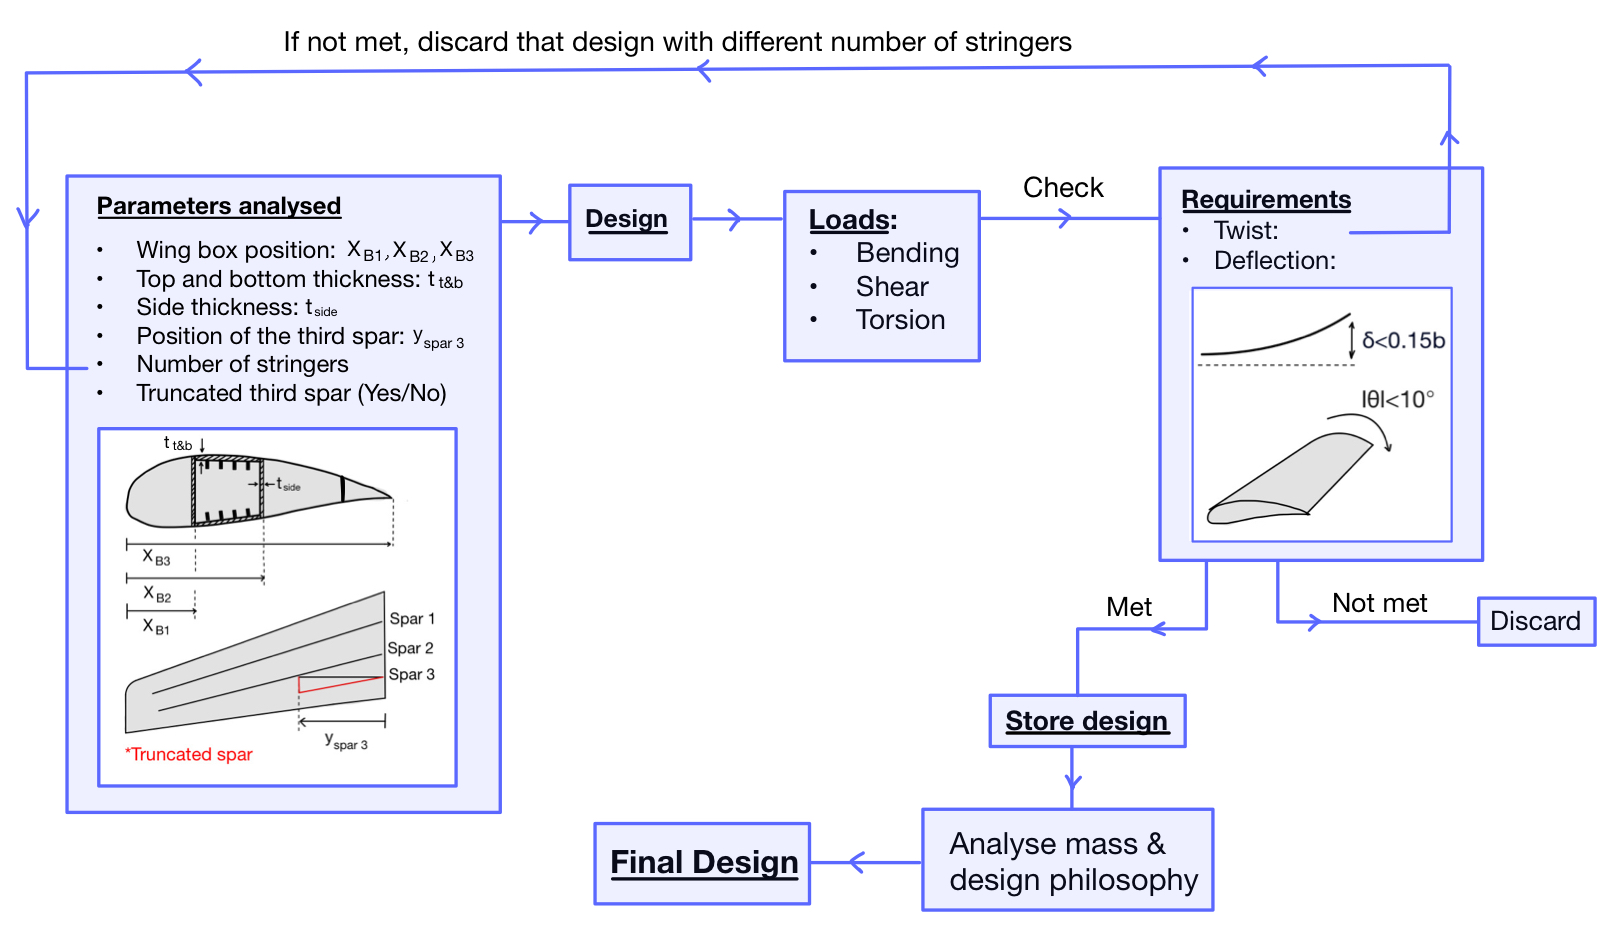
\includegraphics[width=1.1\linewidth]{figures/diagram python code.jpeg}
    \caption{Production of designs procedure}
    \label{fig:sketch_designs_procedure}
\end{figure}

\begin{itemize}
    \item Chordwise positioning of the spars 
    \item Thickness of the Spar caps 
    \item Thickness of the shear webs 
    \item Number of stringers 
    \item The spanwise end of the auxiliary, third spar 
    \item Whether the third spar is truncated or not. 
\end{itemize}
    from this we get the cross sectional area of the wingbox at all spanwise points

    2. using the cross section, get centroid, i.XX and i.YY 

    
\section{Results of the Python code}